\documentclass[a4paper,twoside,12pt]{book}
%% === nezbytné balíčky:
\usepackage[T1]{fontenc}    % kódování písma
%\usepackage[IL2]{fontenc}  % kódování písma

\usepackage[utf8]{inputenc}     % vstupní znaková sada tohoto dokumentu: UTF-8
%\usepackage[cp1250]{inputenc}  % vstupní znaková sada tohoto dokumentu: Windows 1250
%\usepackage[latin2]{inputenc}  % vstupní znaková sada tohoto dokumentu: ISO Latin 2

\usepackage[english]{babel} % česky psaná práce, typografická pravidla. Překládejte pomocí "latex.exe" nebo "pdflatex.exe"
%\usepackage{czech} % česky psaná práce. Překládejte pomocí "pdfCSlatex.exe" ("cslatex.exe" asi bude mít problém s balíkem geometry)

\usepackage[a4paper, hmarginratio=3:2]{geometry} % využití A4 stránky a nastavení okrajů (u vazby bude širší)

\usepackage{pdfpages} % pokud nemáte formulář "Zadání bak./dipl. práce" naskenovaný jako PDF, tak ZAKOMENTUJTE
\usepackage[hidelinks]{hyperref} % v PDF budou klikací odkazy ("hidelinks" je nebude rámovat)

 \hypersetup{
     colorlinks=true,
     linkcolor=blue,
     filecolor=blue,
     citecolor = black,      
     urlcolor=cyan,
     }

%% === balíčky, které se mohou hodit:
%\usepackage{encxvlna} % postará se o spojky a předložky, které dle českých pravidel nesmí být na konci řádku. Dokumentace: http://texdoc.net/texmf-dist/doc/generic/encxvlna/encxvlna.pdf (chová se správně k "vnitřku" listings?)

\usepackage{graphicx} % balíček pro vkládání rastrových grafických souborů (PNG apod.)
%\usepackage{epsfig} % balíčky pro vkládání grafických souborů typu EPS
%\usepackage{float} % rozšířené možnosti umístění obrázků

%\usepackage{caption} % pro popisky obrázků, tabulek atd.

\usepackage{tabularx} % rozšířené možnosti tabulek
%\usepackage{tabu} % jiný balík pro rozšířené možnosti tabulek

%\usepackage{listings}  % balíček vhodný pro ukázky zdrojového kódu v~textu práce/příloh. Nutno nastavit! http://ftp.cvut.cz/tex-archive/macros/latex/contrib/listings/listings.pdf
\usepackage{amsmath} % balíček pro pokročilou matematickou sazbu
%\usepackage{color} % pro možnost barevného textu
%\usepackage{fancybox} % umožňuje pokročilé rámečkování

%\usepackage{index} % nutno použít v případě tvorby rejstříku balíčkem makeindex
%\newindex{default}{idx}{ind}{Rejstřík} % zavádí rejstřík v případě použití balíku index

\usepackage{epigraph}
%\ setting the epigraph width
\setlength{\epigraphwidth}{0.8\textwidth}


% Biblatex package for references
\usepackage[sorting=none]{biblatex}
\addbibresource{sample.bib}

% For headers and footers
\usepackage{fancyhdr}

\pagestyle{fancy}
\renewcommand{\chaptermark}[1]{\markboth{#1}{#1}}
\fancyhead[R]{}
\fancyhead[L]{}
\fancyfoot[C]{\thepage}


% path for figures
\graphicspath{{img/}}

% for footnotes in tables
\usepackage{booktabs,caption}
\usepackage[flushleft]{threeparttable}

% for table footnotes and captions
\usepackage{caption}
\usepackage{subcaption}

% for code highlightning
\usepackage{minted}

% for Appendixes
\usepackage[toc,page]{appendix}

% for nomenclature
\usepackage{nomencl}
\makenomenclature

% for printing of units
\usepackage{siunitx}
\sisetup{load-configurations = abbreviations}



\frenchspacing % za větou bude mezislovní mezera (v anglických textech je mezera za větou delší)
\widowpenalty=1000 % "síla" zákazu vdov (= jeden řádek ze začátku odstavce na konci stránky)
\clubpenalty=1000 % "síla" zákazu sirotků (= jeden řádek/slovo z konce odstavce samostatně na začátku stránky)
\brokenpenalty=1000 % "síla" zákazu zlomu stránky za řádkem, který má na konci rozdělené slovo


\topmargin=-15mm      % horní okraj trochu menší
\textwidth=150mm      % šířka textu na stránce
\textheight=240mm     % "výška" textu na stránce


\pagenumbering{arabic} % číslování stránek arabskými číslicemi


\parindent=0pt % odsazení 1. řádku odstavce
\parskip=7pt   % mezera mezi odstavci

\newcommand{\ti}{\textit} % zkrácený příkaz pro kurzívu
\newcommand{\tb}{\textbf} % zkrácený příkaz pro tučné písmo


%% --- zde jsou zavedeny některé "konstanty" - některé musíte změnit! --- %%
\newcommand{\cvut}{Tertiary Professional School, Secondary School}
\newcommand{\fjfi}{The Centre of professional training Sezimovo Ústí}
\newcommand{\program}{Electrotechnics}

\newcommand{\obor}{Mechatronic systems} % změňte, pokud máte jiný obor

\newcommand{\druh}{Thesis} % nebo "Diplomová práce"
\newcommand{\woman}{} % pokud jste ŽENA, ZMĚŇTE na: ...{\woman}{a} (je to do Prohlášení)

\newcommand{\logoCVUT}{
\includegraphics{img/copsu_logo.jpg}} % logo ČVUT -- podle grafického manuálu ČVUT platného od prosince 2016. Pokud nevyhovuje PDF-verze, tak použijte jinou variantu loga: https://www.cvut.cz/logo-a-graficky-manual -> "Symbol a logo ČVUT v Praze"). Pokud chcete logo úplně vynechat, zadejte místo "\includegraphics{...}" text "\vspace{35mm}"

% přesně podle formuláře "Zadání bak./dipl. práce" VYPLŇTE:
\newcommand{\nazevcz}{Postprocesor robota pro metodu Laser Shock Peening}    % český název práce (přesně podle zadání!)
\newcommand{\nazeven}{Robot post processor for Laser Shock Peening technique}          % anglický název práce (přesně podle zadání!)
\newcommand{\autor}{Marek Böhm}   % vyplňte své jméno a příjmení (s akademickým titulem, máte-li jej)
\newcommand{\vedouci}{Mgr. Bc. Miroslav V. Hospodářský} % vyplňte jméno a příjmení vedoucího práce, včetně titulů, např.: Doc. Ing. Ivo Malý, Ph.D.
\newcommand{\pracovisteVed}{VOŠ, SŠ, COP Sezimovo Ústí} % ZMĚŇTE, pokud vedoucí Vaší práce není z KSI
\newcommand{\konzultant}{Ing. Jakub Horáček} % POKUD MÁTE určeného konzultanta, NAPIŠTE jeho jméno a příjmení
\newcommand{\pracovisteKonz}{HiLASE centrum, Fyzikální ústav AV ČR, v. v. i.} % POKUD MÁTE konzultanta, NAPIŠTE jeho pracoviště

% podle skutečnosti VYPLŇTE:
\newcommand{\rok}{2021}  % rok odevzdání práce (jen rok odevzdání, nikoli celý akademický rok!)
\newcommand{\kde}{Sezimovo Ústí} % studenti z Děčína ZMĚNÍ na: "Děčíně" (doplní se k "prohlášení")

\newcommand{\klicova}{RoboDk, Industrial Robots, Robotic Arms, Collision Avoidance, Simulation, Post processor}   % zde NAPIŠTE česky max. 5 klíčových slov
\newcommand{\keyword}{RoboDk, Industrial Robots, Robotic Arms, Collision Avoidance, Simulation, Post processor}       % zde NAPIŠTE anglicky max. 5 klíčových slov (přeložte z češtiny)
\newcommand{\abstrCZ}{Popis práce česky}    % zde NAPIŠTE abstrakt v češtině (cca 7 vět, min. 80 slov)
\newcommand{\abstrEN}{
The focus of this thesis is to develop a post-processor for the Laser Shock Peening Technique. 

This thesis seeks to answer the following thing: How can a post-processor be altered to use it for the Laser Shock Peening Technique. 

The RoboDK CAM program is a powerful tool that enables users to create their post-processors. In this thesis, the process of modifying a post-processor is described. The post-processor is then tested on a real industrial robotic arm.

} % zde NAPIŠTE abstrakt v angličtině

\newcommand{\prohlaseni}{I declare that I have prepared my thesis independently, and I have used only the materials (literature, projects, software, etc.) listed in the attached list.} % text prohlášení můžete mírně upravit :-)

\newcommand{\podekovani}{I want to thank my supervisor Mgr. Bc. Miroslav V. Hospodářský for the invaluable advice and help in creating this thesis.} % NAPIŠTE poděkování, např. svému vedoucímu:
% Děkuji Ing. Eleonoře Krtečkové, Ph.D. za vedení mé bakalářské práce a za podnětné návrhy, které ji obohatily.
% NEBO:
% Děkuji vedoucímu práce doc. Pafnutijovi Snědldítětikaši, Ph.D. za neocenitelné rady a pomoc při tvorbě bakalářské práce.


%%%%%%%%%%% ZAČÁTEK DOKUMENTU %%%%%%%%%%%
\begin{document}
% start roman numbering in document 
\frontmatter
%%%%%%%%%%%% TITULNÍ STRANA -- na následujících cca 30 řádků NESAHEJTE!!!  Generuje se AUTOMATICKY %%%%%%%%%%%%
\thispagestyle{empty}

\begin{center}
	{\LARGE
		\cvut\par
		\fjfi
	}
    \vspace{10mm}

    \begin{tabular}{c}
		\tb{Program: \program}  \\[3pt]   
		\tb{Specialization: \obor}\\
    \end{tabular}

   \vspace{10mm} \logoCVUT \vspace{15mm} 

   {\huge \tb{\nazevcz}\par}
   \vspace{5mm}   
   {\huge \tb{\nazeven}\par}
   
   \vspace{15mm}
   {\Large \MakeUppercase{\druh}}

   \vfill
   {\large
    \begin{tabular}{ll}
    Author : & \autor\\
    Supervisor: & \vedouci\\
    Year: & \rok
    \end{tabular}
   }
\end{center}

\clearpage{\pagestyle{empty}\cleardoublepage} % prázdná stránka za tou "titulní", bez čísla



%%%%%%%%%%%% ZADÁNÍ PRÁCE %%%%%%%%%%%%
% Zadání (podepsané děkanem!) musíte NASKENOVAT. Ideálně jako 2stránkové PDF (soubor "zadani_cele.pdf"). 
% Před svázáním to v jednom výtisku VYMĚNÍTE ZA ORIGINÁLNÍ ZADÁNÍ (podepsané děkanem fakulty)!
\newpage  % SEM NESAHEJTE!
\thispagestyle{empty} % SEM NESAHEJTE!

%% zde podle toho, jak jste zadání naskenovali, VYBERTE variantu A, B nebo C:
%
% --- varianta A: zadání naskenované jako 2stránkové PDF:
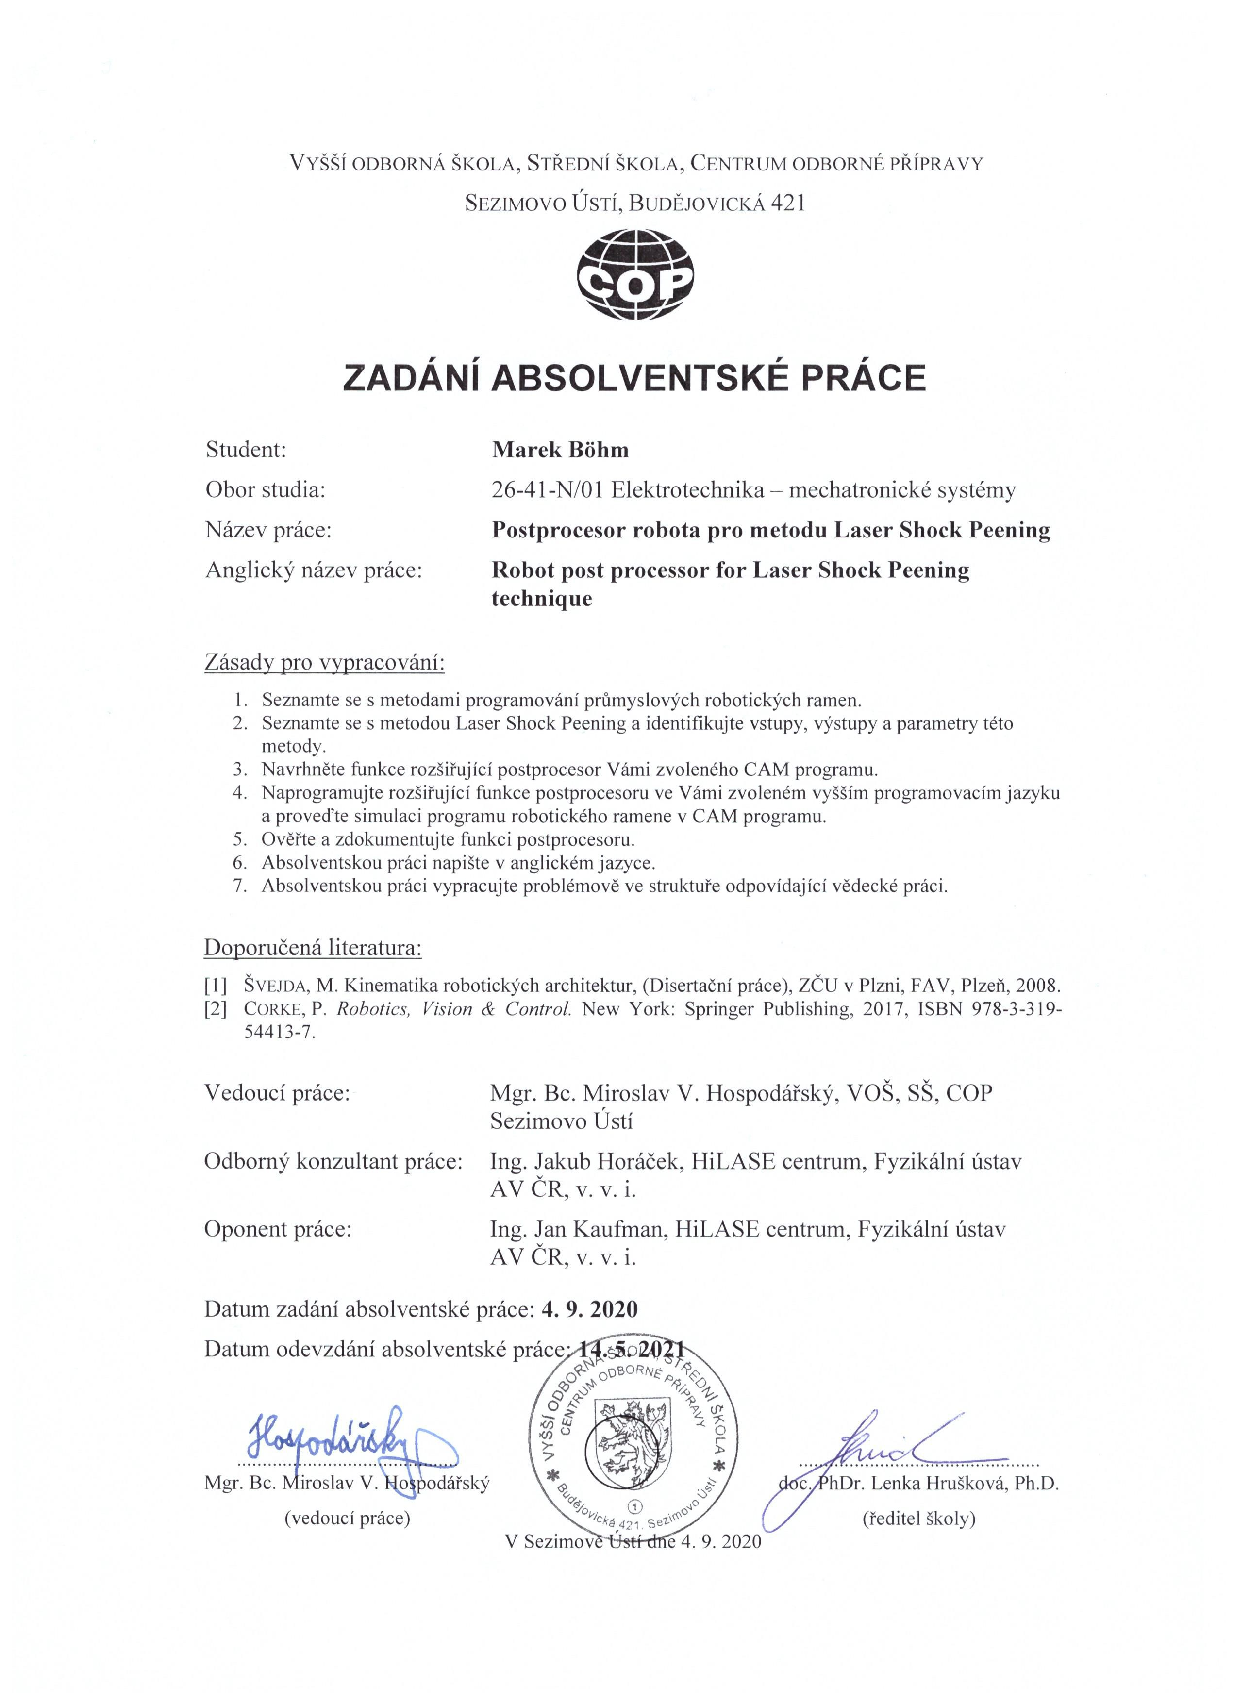
\includepdf[pages={1}]{assignment/assignment_scan.pdf} % NAHRAĎTE správným souborem!
%
%% --- varianta B: zadání naskenované jako jednotlivé stránky:
%\includepdf[pages={1}]{zadani1.pdf} % 1. strana zadání v PDF
%\includepdf[pages={1}]{zadani2.pdf} % 2. strana zadání v PDF
%
%% --- varianta C: zadání naskenované jako 2 samostatné obrázky:
%% 1. strana zadání
%\begin{center}
%     \includegraphics[width=1\textwidth]{zadani1.jpg}
%\end{center}
%% 2. strana zadání
%\newpage  % SEM NESAHEJTE!
%\thispagestyle{empty} % SEM NESAHEJTE!
%\begin{center}
%     \includegraphics[width=1\textwidth]{zadani2.jpg}
%\end{center}


%%%%%%%%%%%% Prohlášení -- SEM NESAHEJTE! Generuje se automaticky z výše nastavených maker \kde{} a \prohlaseni{}. %%%%%%%%%%%%
\newpage % SEM NESAHEJTE!
\thispagestyle{empty}  % SEM NESAHEJTE!

~ % SEM NESAHEJTE!
\vfill % prázdné místo. SEM NESAHEJTE!

\tb{Declaration} % SEM NESAHEJTE!

\vspace{1em} % vertikální mezera. SEM NESAHEJTE!
\prohlaseni

\vspace{2em}  % SEM NESAHEJTE!
\hspace{-0.5em}\begin{tabularx}{\textwidth}{X c}  % SEM NESAHEJTE!
In \kde\ on .................... &........................................ \\	% SEM NESAHEJTE!
	& \autor
\end{tabularx}	% SEM NESAHEJTE!


%%%%%%%%%%%% Poděkování  %%%%%%%%%%%%
\newpage
\thispagestyle{empty}

~
\vfill % prázdné místo


% -- následující kus kódu (do "%%%%%%%%%%%% ABSTRAKT") můžete odstranit, pokud nechcete psát poděkování:
\tb{Acknowledgments}

\vspace{1em} % vertikální mezera
\podekovani
\begin{flushright}
\autor
\end{flushright}  % <------- tady končí stránka s poděkováním


%%%%%%%%%%%% ABSTRAKT atp. Je generován AUTOMATICKY podle maker nastavených na začátku souboru) %%%%%%%%%%%% 
\newpage   % SEM NESAHEJTE!
\thispagestyle{empty}   % SEM NESAHEJTE!

% příprava:    (na následujících 8 řádků NESAHEJTE!)
\newbox\odstavecbox
\newlength\vyskaodstavce
\newcommand\odstavec[2]{%
    \setbox\odstavecbox=\hbox{%
         \parbox[t]{#1}{#2\vrule width 0pt depth 4pt}}%
    \global\vyskaodstavce=\dp\odstavecbox
    \box\odstavecbox}
\newcommand{\delka}{120mm} % šířka textů ve 2. sloupci tabulky

% použití přípravy:    % dovnitř "tabular" vůbec NESAHEJTE!
\begin{tabular}{ll}
  {\em Název práce:} & ~ \\
  \multicolumn{2}{l}{\odstavec{\textwidth}{\bf \nazevcz}} \\[1em]
  {\em Autor:} & \autor \\[1em]
  {\em Studijní program:} & \program \\
  {\em Obor:} & \obor \\
  {\em Druh práce:} & \druh \\[1em]
  {\em Vedoucí práce:} & \odstavec{\delka}{\vedouci\\ \pracovisteVed} \\
  {\em Konzultant:} & \odstavec{\delka}{\konzultant \\ \pracovisteKonz}  % VYMAŽTE text "-- %" v případě, že jste neměli konzultanta
 \\[1em]  
  \multicolumn{2}{l}{\odstavec{\textwidth}{{\em Abstrakt:} ~ \abstrCZ  }} \\[1em]
  {\em Klíčová slova:} & \odstavec{\delka}{\klicova} \\[2em]

  {\em Title:} & ~\\
  \multicolumn{2}{l}{\odstavec{\textwidth}{\bf \nazeven}}\\[1em]
  {\em Author:} & \autor \\[1em]
  \multicolumn{2}{l}{\odstavec{\textwidth}{{\em Abstract:} ~ \abstrEN  }} \\[1em]
  {\em Key words:} & \odstavec{\delka}{\keyword}
\end{tabular}



%%%%%%%%%%%% Obsah práce ... je generován AUTOMATICKY %%%%%%%%%%%%
\newpage  % SEM NESAHEJTE!
\parskip=0pt
\tableofcontents % SEM NESAHEJTE!
\parskip=7pt
\newpage % SEM NESAHEJTE!

\mbox{}

\nomenclature{$c$}{Speed of light in a vacuum inertial frame}
\nomenclature{$h$}{Planck constant}

\cleardoublepage
\addcontentsline{toc}{chapter}{Nomenclature}
\printnomenclature


\cleardoublepage
% \phantomsection
\addcontentsline{toc}{chapter}{\listfigurename}
\listoffigures

\cleardoublepage
% \phantomsection
\addcontentsline{toc}{chapter}{\listtablename}
\listoftables

%--------------------------------------------------------
%|         Zde začíná SAMOTNÁ PRÁCE (text)              |
%--------------------------------------------------------

\chapter*{Introduction} % SEM NESAHEJTE!
\addcontentsline{toc}{chapter}{Introduction} % SEM NESAHEJTE!

\pagestyle{fancy}
\renewcommand{\chaptermark}[1]{\markboth{#1}{#1}}
\fancyhead[R]{\chaptername\ \thechapter\ --\ \leftmark}
\fancyhead[L]{}


%
Zde napište text úvodu (1-3 strany, nerozdělujte na podkapitoly) nebo jej vložte ze samostatného souboru: např. příkazem \texttt{\textbackslash input\{vnitrek\_uvod.tex\}}.
%

%\input{vnitrek_kapitola1.tex} % text vkládán ze souboru. Pokud je v souboru uveden i příkaz \chapter{...}, tak ho o 4 řádky výše vymažte.

% arabic numbering
\mainmatter

\chapter{Basics of industrial robots}

\epigraph{

Excerpt from the play Rossum’s Universal Robots (RUR).\break
In the introductory scene Helena Glory is visiting Harry Domin the director general of Rossum’s Universal Robots and his robotic secretary Sulla.\break
\break
\textbf{Domin:} Sulla, let Miss Glory have a look at you.\break
\textbf{Helena (stands and offers her hand):} Pleased to meet you. It must be very hard for you out here, cut off from the rest of the world [the factory is on an island].\break
\textbf{Sulla:} I do not know the rest of the world Miss Glory. Please sit down.\break
\textbf{Helena (sits):} Where are you from?\break
\textbf{Sulla:} From here, the factory\break
\textbf{Helena:} Oh, you were born here.\break
\textbf{Sulla:} Yes I was made here.\break
\textbf{Helena (startled):} What?\break
\textbf{Domin (laughing):} Sulla isn’t a person, Miss Glory, she’s a robot.\break
\textbf{Helena:} Oh, please forgive me …
}{\textit{Karel Čapek \\ Rossum’s Universal Robots (RUR)}}

\section{Classification of industrial robots and their structures}

Industrial robots can be classified according to various criteria: the number of degrees of freedom, kinematic structure, drives used, workspace geometry, motion characteristics, control method or programming method. According to the abovementioned criteria, several types of robots are distinguished:

\subsection*{Number of degrees of freedom}

\begin{itemize}
    \item Universal robot - 6 degrees of freedom
    \item Redundant robot - more than 6 degrees of freedom
    \item Deficient robot - less than 6 degrees of freedom
\end{itemize}

\subsection*{Kinematic structure}

\begin{itemize}
    \item Serial robots - with an open-loop kinematic chain
    \item Parallel robots - with a closed-loop kinematic chain
    \item Hybrid robots - combining both types of kinematic chains
\end{itemize}


\subsection*{Type of drives}

\begin{itemize}
    \item Electric
    \item Hydraulic
    \item Pneumatic
\end{itemize}

Currently, industrial robots with electric drives predominate in numbers. If high loads are required, hydraulic drives are used and for high speeds pneumatic drives are preferred.

\subsection*{Workspace geometry}

\begin{itemize}
    \item Cartesian
    \item Cylindrical
    \item Spherical
    \item Angular
    \item SCARA
\end{itemize}

\section{Industrial robot programming}

Before we dive into the programming of industrial robotic arms, let us revise a few concepts.
A workcell represents a robot and a collection of machines or peripherals. A single robot controller is responsible for controlling the various appliances of a workcell.

A robot end effector is a peripheral placed at the end of the robotic arm. The end effector represents the last link of the robot. According to the application, end effectors can be grippers, welding devices, spray guns or grinding and deburring machines.

The robot controller is equipped with a so-called interface software. The interface software makes it easier for the user to program the robotic arm.  
Two basic information need to be programmed into the robotic arm:

\begin{itemize}
    \item position data 
    \item procedure
\end{itemize}

Many different ways of teaching a robot position do exist:

\begin{itemize}
    \item Positional commands
    \item Teach pendant
    \item Lead-by-the-nose
    \item Offline programming
    \item Robot simulation tools
    \item Manufacturing independent robot programming tools
\end{itemize}

\subsection{Offline programming}
Different robot brands have incompatible interfaces. Robot programming languages evolve slowly, and robot manufacturers offer backwards compatibility. For example, FANUC ...

Offline programming  (OLP) refers to a programming method in which the robot is programmed outside the production environment. OLP helps to eliminate production downtime, allows studying multiple scenarios of a robot cell before setting up the productions cell. OLP also aids in predicting mistakes made in designing a work cell.


\chapter{Laser Shock Peening}

    \epigraph{Since the early middle ages, mankind has always struggled to increase the hardness and flexibility of metals, to improve the durability and reliability of  metal tools and parts. From the damascus steel smiths through the swordsmiths of medieval japan, the method of cold-working metal by the application of precise mechanical pressure such as hammer blows has a glorious history.

In modern times, this concept has reached its apex with industrial surface hardening using shot peening, where thousands of small lead shot are fired at the metal surface, compressing and hardening the surface , improving the durability. With the advent of high power laser systems, an improved process has been developed, the process of Laser Shock peening.}{\textit{Samuel Zhrdne\\ HoloOr company}}

\section{Laser Shock Peening}

Laser Shock Peening (LSP) treatment induces residual stresses beneath the treated surface of metallic materials. The residual stresses are produced by a high magnitude shock wave induced by a high-energy laser pulse. The advantage of LSP is that the laser pulse can be adjusted and controlled in real time. A computer-controlled system can measure the energy per pulse and record it for each LSP process on the component \cite{mannava}.

\subsection{Laser Shock Peening Process}
The configuration of an LSP process on a metallic component is shown in Figure \ref{fig:lspconfiguration}. An intense pulsed laser shock beam is fired onto a metal surface for a brief time (\SIrange{10}{100}{\ns}). The heated zone is vaporized and transformed to plasma by ionization due to high temperatures (over \SI{10000}{\degreeCelsius} ). The plasma is under high pressure, which propagates through the material via shock waves. Two modes of LSP exist – the direct ablation mode and the confined ablation mode. The direct ablation mode refers to the interaction of plasma with metal without coating and confinement \cite{sano}. Plasma pressure of tenths of a \SI{}{\GPa} is achieved using direct ablation mode. Higher pressures of \SIrange{1}{5}{\GPa} can be obtained using the confined mode. In the confined mode, the metal surface is usually coated with an opaque material such as black paint or aluminium foil and confined by a material transparent to the laser radiation such as distilled water or borosilicate glass. A stronger pressure pulse results in a higher magnitude of compressive residual stress to a deeper depth \cite{fairland}.

\begin{figure}[h]
    \centering
    
\includegraphics[width=0.6\linewidth]{img/lsp_configuration.jpg}
    \caption{Schematic configuration of laser shock peening}
    \label{fig:lspconfiguration}
\end{figure}

\subsection{Laser Shock Peening Strategy}
During the peening process, a pattern is created made of individual laser pulses. Generally, multiple sequences of the pattern that are gradually shifted across the sample are used to create a layer, as seen in Figure \ref{fig:lspstrategy}. The pattern shifting ensures a more homogeneous residual stress distribution. This peening strategy's disadvantage is that the protective coating needs to be replaced in between sequences \cite{kaufman}.

\begin{figure}[h]
    \centering
    
\includegraphics[width=0.6\linewidth]{img/lsp_strategy.jpg}
    \caption{Laser shock peening strategy - one layer consisting of four sequences}
    \label{fig:lspstrategy}
\end{figure}

\section{LSP station and laser source at HiLASE Centre}

The LSP station uses the Bivoj laser system, located on the ground floor of the HiLASE Centre. The HiLASE Research Centre is an excellent pan-European infrastructure in laser research and development, located in Dolní Břežany, Czech Republic. The logo of the HiLASE Centre is shown in Figure A Laser Beam Distribution System (LBDS) transports the beam to
experimental laboratory on the 1\textsuperscript{st} floor. The Bivoj laser system is a Diode Pumped Solid State Laser (DPSSL) based on Yb-doped gain media with a laser wavelength of 1030 nm capable of delivering energy pulses up to \SI{8}{\joule} at a \SI{10}{\hertz} repetition rate. The beam shape at the output of the Bivoj laser is a square flat-top pulse. An overview of the BIVOJ laser system is shown in Figure \ref{fig:bivoj}. The two main sections of the Bivoj laser are the front-end and the \SI{10}{\joule} amplifier.



\begin{figure}[h]
    \centering
    
\includegraphics[width=0.6\linewidth]{img/hilase.jpg}
    \caption{Logo of HiLASE Centre.}
    \label{fig:lspconfiguration}
\end{figure}

\begin{figure}[h]
    \centering
    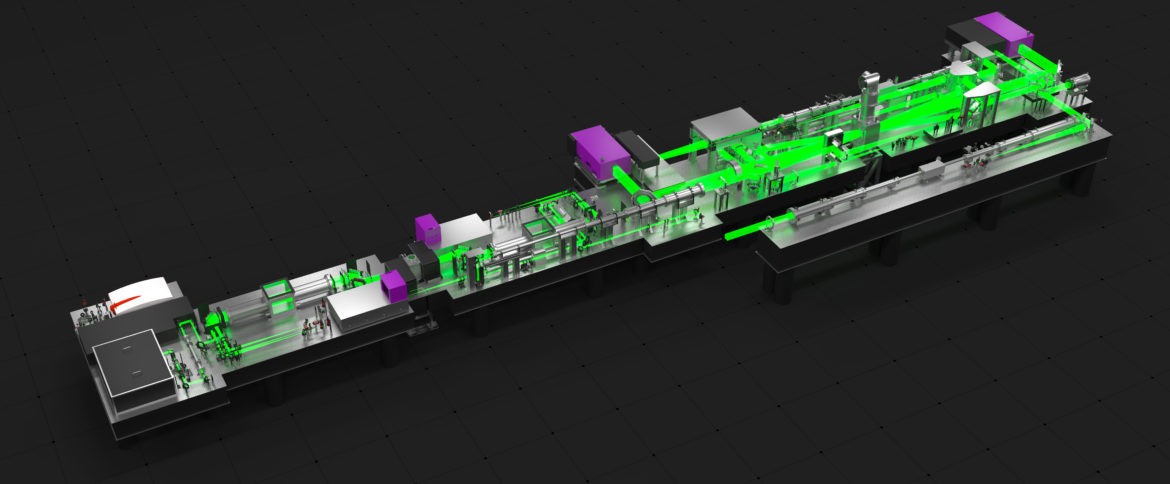
\includegraphics[width=1.0\linewidth]{img/bivoj.jpg}
    \caption{Laser system "BIVOJ": Diode-pumped solid-state (DPSSL) laser DiPOLE 100}
    \label{fig:bivoj}
\end{figure}

\subsection{Bivoj laser system}

\subsubsection*{Bivoj front-end}

The front end starts with a fibre-based section, consisting
of a fibre oscillator, fibre amplifier and temporal pulse shaper
with \SI{125}{\ps} resolution. The output of the fibre front-end is fed
to the first booster amplifier, which is regenerative and
increases the energy to \SI{30}{\milli\joule} and reduces the repetition rate to \SI{10}{\hertz}. The second booster amplifier works in a multi-pass regime
and increases the pulse energy to approximately \SI{30}{\milli\joule}.
The repetition rate can be switched between \SI{1}{\hertz} and \SI{10}{\hertz}. The
beam shape at the front-end output is \SI{8 x 8}{\mm\squared} square flat top.

\subsubsection*{Bivoj 10 J amplifier}

The \SI{10}{\joule}  amplifier is the first-stage main amplifier based on
cryogenically cooled multi-slab technology. The principal
component of the amplifier is the amplifier head, where the
gain media are stored and cooled by gaseous helium to 
the temperature of about \SI{150}{\kelvin}. The laser beam from the front-end
is enlarged to \SI{22 x 22}{\mm\squared} and sent to the \SI{10}{\joule} amplifier, where
increases its pulse energy from approximately \SI{30}{\milli\joule} to
approximately \SI{8}{\joule} at \SI{10}{\hertz}. The spatial profile of the laser beam at the output of the BiVOJ \SI{10}{\joule} amplifier is shown in Figure \ref{fig:spatialprofile} and the temporal profile is shown in Figure \ref{fig:temporalprofile} \cite{saumyabrata}.

\begin{figure}[h]
    \centering
    
\includegraphics[width=0.6\linewidth]{img/spatial_profile.jpg}
    \caption{Spatial profile of laser beam at output of BiVOJ \SI{10}{\joule} amplifier and approximate dimensions.}
    \label{fig:spatialprofile}
\end{figure}

\begin{figure}[h]
    \centering
    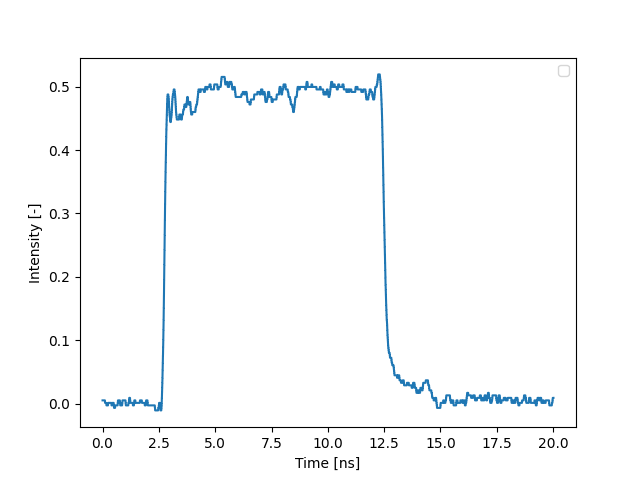
\includegraphics[width=0.6\linewidth]{img/temporal_profile_bivoj.png}
    \caption{Temporal profile of laser beam at output of BiVOJ \SI{10}{\joule}.}
    \label{fig:temporalprofile}
\end{figure}

\subsection{Litron LPY ST 7875-10 2HG laser}

The second laser source available at the LSP station is the Litron LPY ST 7875-10 2HG laser, a tabletop laser located directly in the experimental laboratory next to the LSP station. This laser is a pulsed Q-switched Nd:YAG laser suited for industrial or research applications. The Litron  LPY ST 7875-10 2HG laser comes with a Super-Gaussian resonator. The most critical parameters of this system are highlighted in Table \ref{litronparameters} and the laser system is shown in Figure \ref{fig:litron} \cite{litron}. 


\begin{table}[h!]
\centering
    \begin{threeparttable}
        \begin{tabular}{||c | c||} 
        \hline
            \textbf{Parameter} & \textbf{Value} \\ [0.5ex] 
        \hline\hline
        Repetition Rate [Hz] & 10  \\ 
        \hline
            Output Energy [mJ] & \\
            1064nm & 3500 \\
            532nm & 1750 \\
        \hline
            Beam Diameter [mm] & 15 \tnote{a} \\
        \hline
            Beam Divergence [mrad] & <0.5 \tnote{b} \\ 
        \hline
            Pulse Length @1064nm [ns] & 10-12 \\
        \hline
            Pointing Stability [µrad] & 25 \tnote{c} \\
        \hline
            Timing Jitter [ns] & <0.5 \tnote{d}  \\
        \hline
        \hline
        \end{tabular}
        \begin{tablenotes}
            \small
            \item[a] Peak-to-peak Energy - 99 \% of pulses. 
            \item[b] Full angle for 90 \% of the energy.
            \item[c] Half angle.
            \item[d] Jitter is measured concerning the external Q-switch trigger input.
        \end{tablenotes}
    
        \caption{Litron LPY ST 7875-10 2HG parameters}
        \label{litronparameters}
    \end{threeparttable}
\end{table}

\begin{figure}[h]
    \centering
    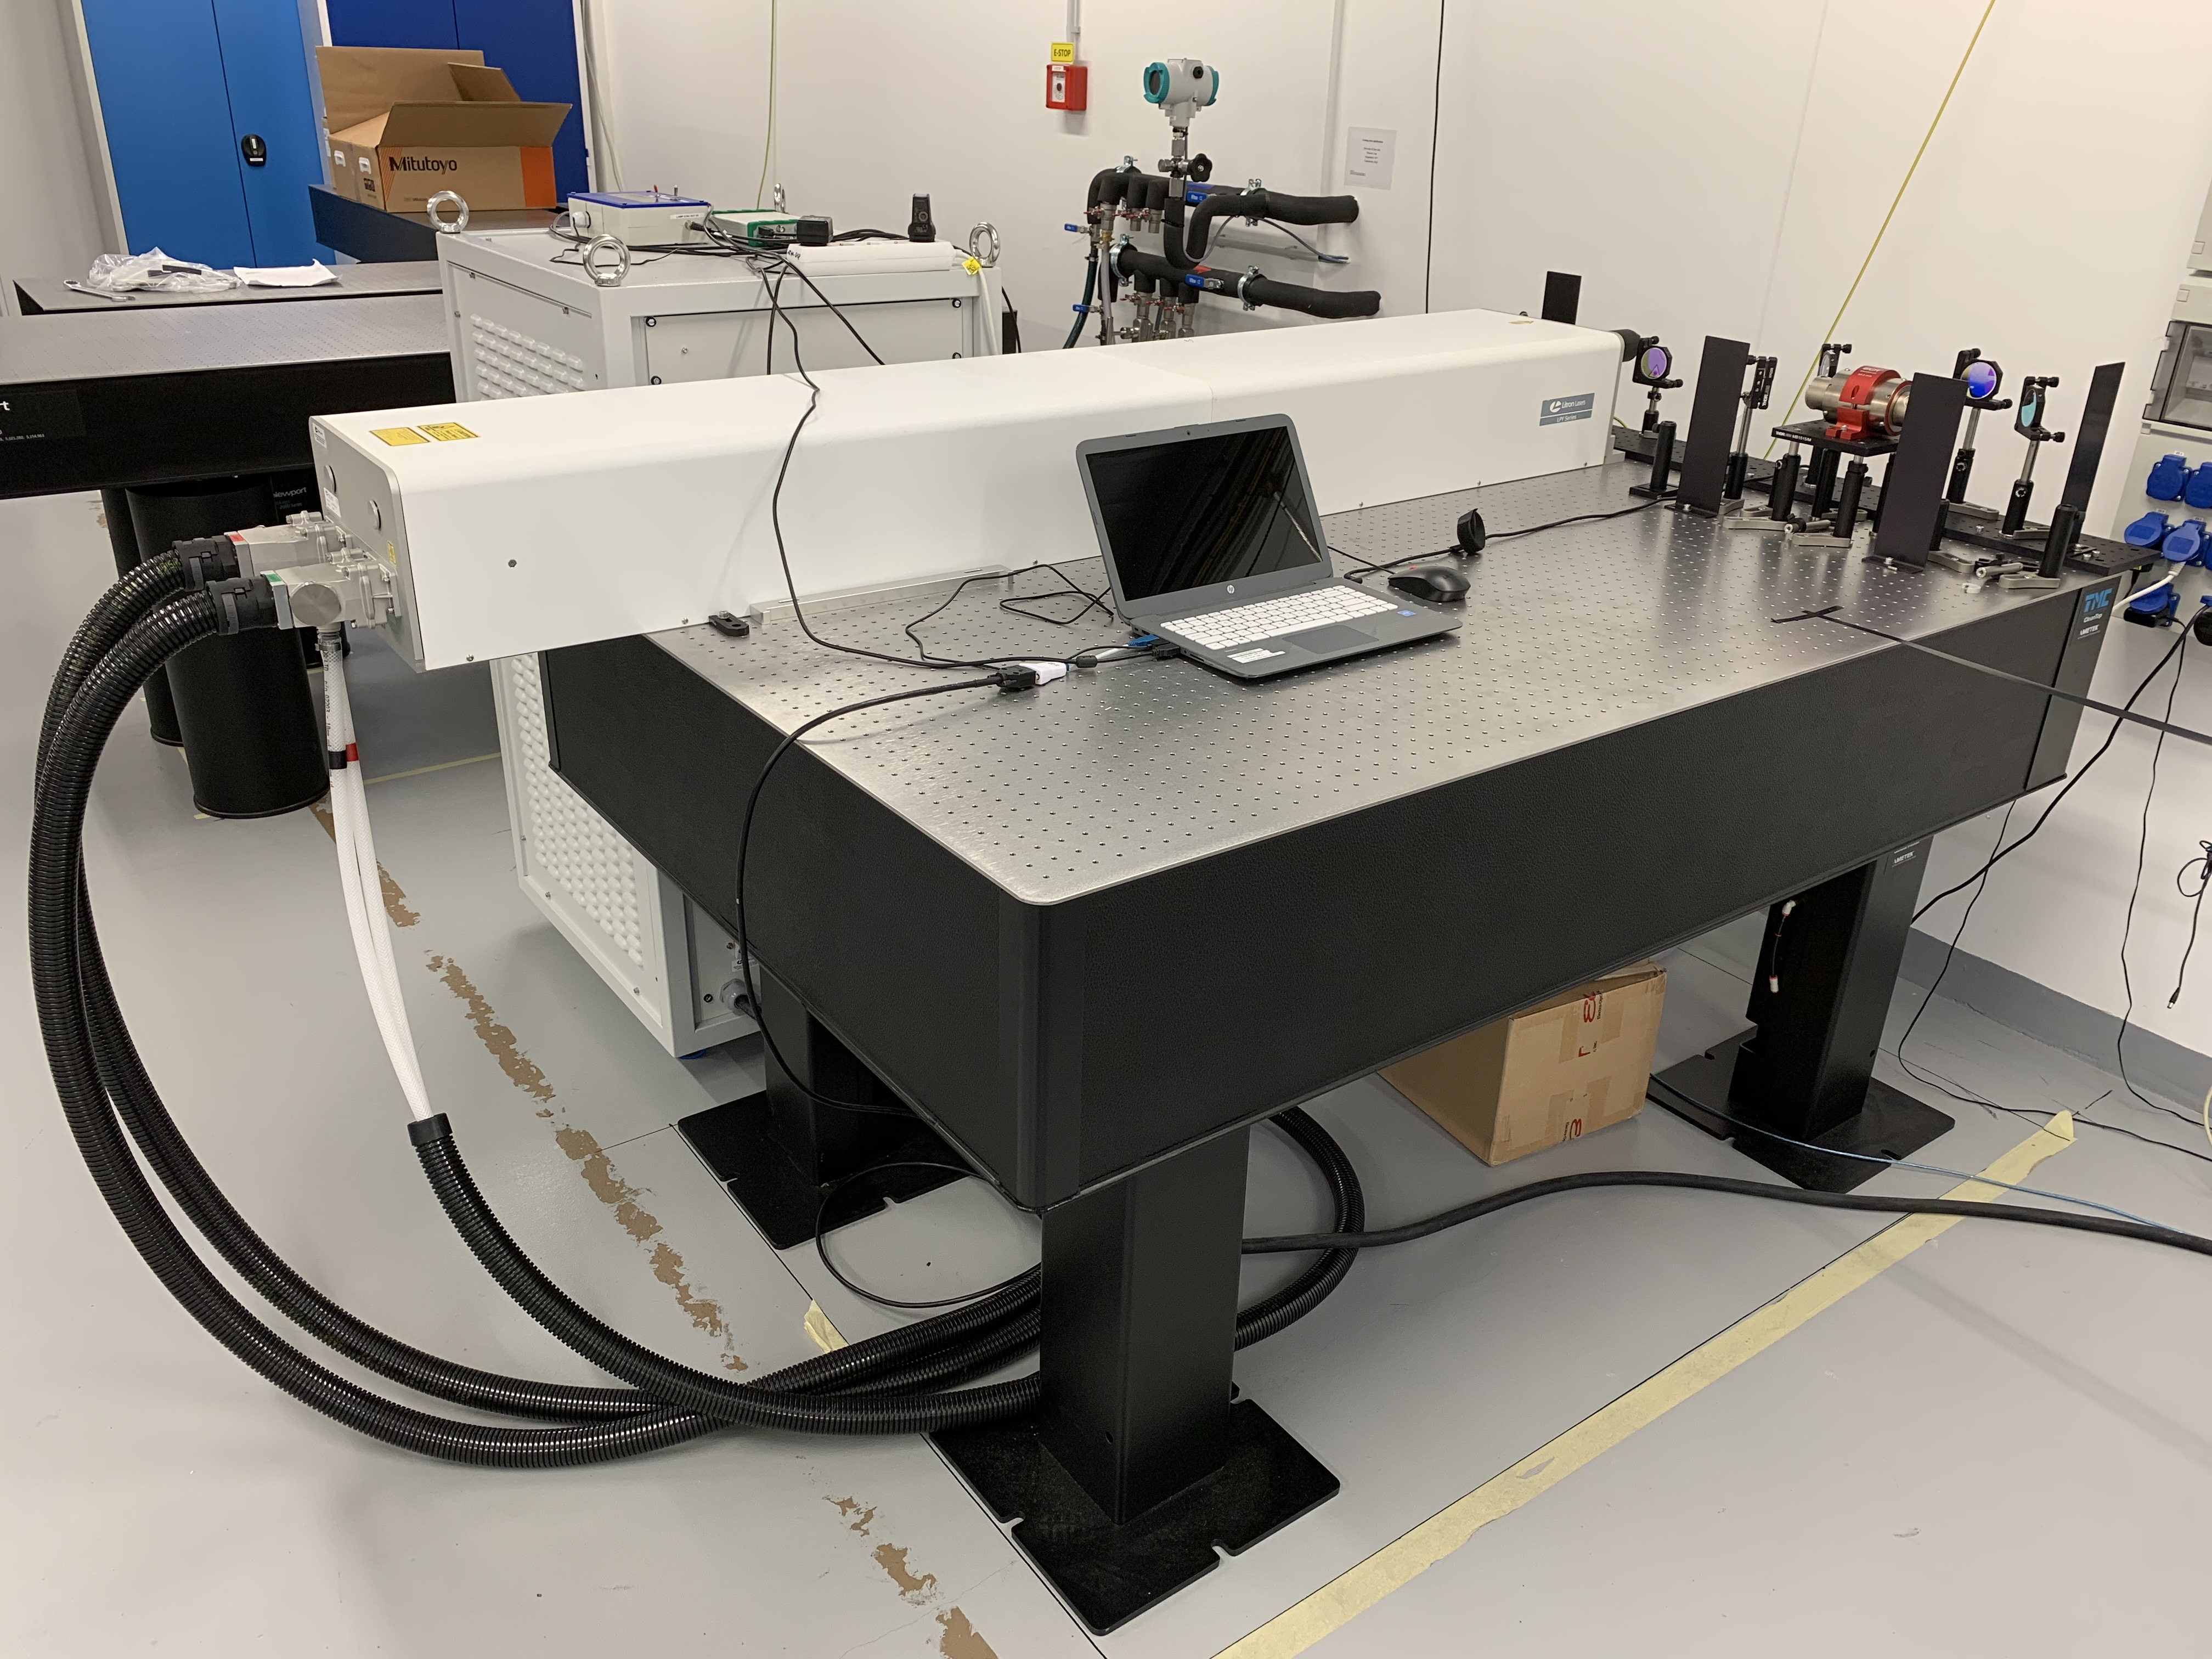
\includegraphics[width=0.6\linewidth]{img/litron.JPG}
    \caption{Litron LPY ST 7875-10 2HG laser at HiLASE Centre.}
    \label{fig:litron}
\end{figure}



\subsection{LSP station layout}

The layout of the LSP station is as shown in Figure \ref{fig:lsplayout}. The laser
beam enters the LSP station through the LSP output node and
continues to the optical table, where it is redirected and
focused on the target. The target itself is mounted on the
robotic arm. The laser beam position is fixed, so the robotic
arm needs to be moved to direct the laser.

\begin{figure}[t!]
\centering
\begin{subfigure}{.45\textwidth}

    
\includegraphics[width=1\linewidth]{img/lsp_layout.jpg}

    \label{fig:a}
\end{subfigure}
\begin{subfigure}{.45\textwidth}

    \includegraphics[width=1\linewidth]{img/lsp_station_real.JPG}

    \label{fig:b}
\end{subfigure}

\caption{(from left to right)Schematic layout of LSP station and photography of LSP station.}
\label{fig:lsplayout}
\end{figure}

\subsection{FANUC M-20iA/20M robotic arm}

The FANUC M-20iA/20M is a 6-axis universal industrial robotic arm with a maximum load capacity at the wrist of \SI{20}{\kg} and a maximum reach of \SI{1811}{\mm}. The repeatability of the robotic arm is \SI{+-0.08}{\mm} The FANUC M-20iA/20M is a multi-purpose robotic arm and can be used for various applications such as assembling, packaging and machining. The  FANUC M-20iA/20M robot is shown in Figure \ref{fig:fanucrobot} \cite{fanucrobot}.

\begin{figure}[h]
    \centering
    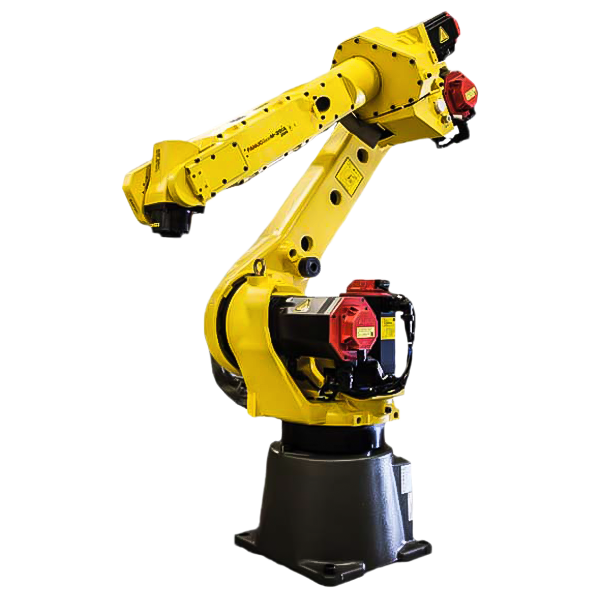
\includegraphics[width=0.6\linewidth]{img/fanuc_robot.png}
    \caption{FANUC M-20iA/20M industrial robotic arm  \cite{fanucrobot}.}
    \label{fig:fanucrobot}
\end{figure}

The robot is coupled with a FANUC R-30iA controller. The R-30iA controller is equipped with a FANUC AIF01A PLC Interface module. The Interface module is connected to the following expansion modules:

\begin{itemize}
    \item AID16L - 16 digital inputs
    \item AOD16D - 16 digital outputs
    \item ADA02A - 2 analog outputs \cite{fanucunitmanual}
\end{itemize}

\subsection{LSP process example}

The following \href{https://www.youtube.com/watch?v=awhlLU91-dk&ab_channel=HiLASECentre}{video} shows the improvement of cavitation erosion Resistance by Laser Shock Peening carried out at HiLASE Centre. This process is developed by HiLASE Center and SIGMA GROUP Plc. for the improvement of cavitation erosion resistance of pump blades. The parameters chosen for this experiment are:



\chapter{Design}

    \epigraph{If you drive a car, it makes little difference what brand it is: all cars are driven
in essentially the same way. The same applies to computers. If you have a
Windows PC, the user interface won’t be affected by your computer hardware.
This is definitely not the case for industrial robots.}{\textit{Albert Nubiola \\ CEO at RoboDK}}

\section{RoboDK overview}

RoboDK (short for Robot Development Kit) is a development platform for industrial robot offline programming and simulation for industrial robots.

\subsection{RoboDK history}

RoboDK (the company) was founded by Albert Nubiola and Lauren Ierullo in January 2015 as a spin-off company from the \href{https://en.etsmtl.ca/unites-de-recherche/coro/accueil?lang=en-CA}{CoRo laboratory}   at ETS University in Montreal, Canada. RoboDK is a commercial version of RoKiSim, a multiplatform educational software tool for 3D simulation of serial 6-axis robots.

\subsection{RoboDK features}


The following section highlights some of the features RoboDK has to offer. 


\begin{itemize}
\item Intuitive graphical user interface
\item Drag-and-drop functionality 
\item Supported 3D models - Importing objects and creating new tools using 3D files such as STL, STEP and IGES
\item External axes - Integrating external axes to extend the robot’s reachability
\item Generating Programs - Generating programs for various robot manufacturers
\item Running programs on the fly – Executing programs directly from an external computer
\item Real-time monitoring – Viewingthe robot state on an external computer 
\item CAM for robots - converting 5-axis CNC toolpaths to robot programs and using a robot like a 5-axis CNC
\item Automated path solving - Avoiding robot errors, including singularities, joint limits, reach limits, and collisions
\item Fast collision detection - Defining the object interactions 
\item Advanced use - Creating robot programs from an external computer using a higher programming language. The RoboDK API is available in Python, C#, Visual Basic, C++, and Matlab
\item Simulating 2D vision cameras - Testing image recognition algorithms in the simulation environment
\item Multiple robot simulation - Synchronizing and programming multiple robots and moving them at the same time 
\item Customizable post processor - Integrating specific sensors or actuators such as grippers, force control, image processing, etc.
\end{itemize}

\subsection{RoboDK licences and versions}

RoboDK offers a free (limited), educational or professional version. 
The software is available for Windows, Mac OS, Ubuntu Linux or Android. It supports either 32 or 64-bit versions of the abovementioned operating systems. At the time of writing this document, the latest version of RoboDK is 5.2. The complete RoboDK revision history is available online at this \href{https://en.etsmtl.ca/unites-de-recherche/coro/accueil?lang=en-CA}{link}. The logo of RoboDK is shown in Figure \ref{fig:robodklogo}.

\begin{figure}[h]
    \centering
    
\includegraphics[width=0.6\linewidth]{img/robodk_logo.png}
    \caption{RoboDK logo.}
    \label{fig:robodklogo}
\end{figure}

\section{RoboDK robot library}

RoboDK supports offline programming and has an extensive robot library supporting many robot controllers, including:

\begin{itemize}
    \item ABB RAPID (mod/prg)
    \item Fanuc LS (LS/TP)
    \item KUKA KRC/IIWA (SRC/java)
    \item Motoman Inform (JBI)
    \item Universal Robots (URP/script)
\end{itemize}
Models of industrial robots in RoboDK have the same properties as used with an actual robotic controller. The RoboDK library can be accessed either online via this \href{https://en.etsmtl.ca/unites-de-recherche/coro/accueil?lang=en-CA}{link}  or in the RoboDK application itself. 



\section{RoboDK interface}

The interface of RoboDK consists of the main menu, the toolbar, the station tree, the status bar, and the 3D view. A picture of the RoboDK interface is shown in Figure \ref{fig:robodkinterface}. An extensive documentation for RoboDK is available online via this \href{https://robodk.com/doc/en/Basic-Guide.html#Start}{link}.

\subsection{RoboDK station}

A RoboDK project containing a robot, robot tools, additional CAD files, robot frames and a robot program is called a station. A RoboDK station is saved as one file (\mintinline{shell-session}{.rdk} extension).  The FANUC M-20iA/35M is used in this thesis because it is readily available in the RoboDK library and differs from the FANUC M-20iA/20M robotic arm only in payload capacity.

\begin{figure}[h]
    \centering
    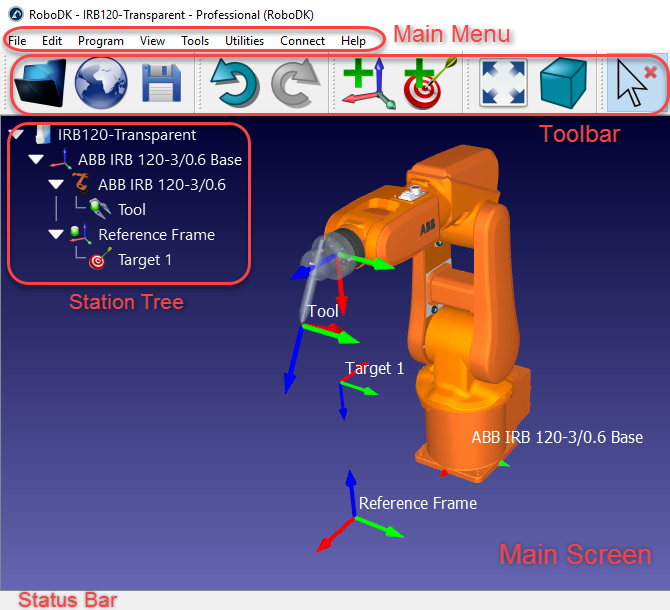
\includegraphics[width=0.9\linewidth]{img/robodk_interface.png}
    \caption{RoboDK interface v 5.0 running on Windows 10.}
    \label{fig:robodkinterface}
\end{figure}

\section{RoboDK API}

RoboDK provides a GUI to simulate and program industrial robots. No programming experience is required to simulate and program robots using the GUI. Unfortunately, the GUI has some limitations for simulation and offline programming. Then the RoboDK API can extend the capabilities of RoboDK using a programming language such as Python.

The API exposes a set of routines and commands to RoboDK, enabling the user to program the robot using high-level programming languages. The RoboDK API is available for Python, C#, C++, Visual Basic (.NET) and Matlab. Any of these programming languages can be used to simulate and program any robot arm. The API can conveniently handle the following tasks:

\begin{itemize}
    \item Automating the simulation
    \item Offline programming
    \item Online Programming
\end{itemize}

The RoboDK API is divided into the following modules:


\begin{itemize}
    \item \mintinline{shell-session}{robolink} module - this module represents the link between RoboDK and the programming language
    \item \mintinline{shell-session}{Item} module - any item from the RoboDK item tree can be retrieved.  An item can be a robot, a reference frame, a tool, an object or a specific project.
    \item \mintinline{shell-session}{robodk} module - a module with a robotics toolbox for pose operations.All post processors depend on the robodk module.
\end{itemize}

\section{RoboDK Plug-Ins}

\subsection{RoboDK Plug-In interface}

Plug-Ins can extend RoboDK's functionality. Plug-Ins can be developed by using the RoboDK Plug-In interface. The RoboDK Plug-In interface is linked natively to the core of RoboDK. Examples of RoboDK Plug-Ins are available at this \href{https://github.com/RoboDK/Plug-In-Interface}{link}. 

\subsection{RoboDK Plug-In for SolidWorks}

\begin{figure}[h]
    \centering
    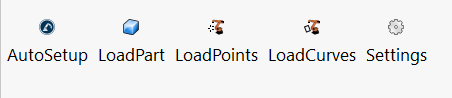
\includegraphics[width=0.6\linewidth]{img/solidworks_toolbar.PNG}
    \caption{SolidWorks RoboDK Plug-In Toolbar.}
    \label{fig:solidworkstoolbar}
\end{figure}


Solidworks is a professional 3D CAD modelling application. The RoboDK Add-in for SolidWorks allows to combine SolidWork's 3D CAD modelling features with RoboDK for robot simulation and offline programming and considerably simplifies the programmer's workflow. The programmed can load 3D models created in SolidWorks directly to RoboDK. Groups of curves and point can also be loaded to RoboDK, and robot programs can be generated from them.

\subsubsection*{SolidWorks RoboDK Plug-In Toolbar}

After opening SolidWorks under the RoboDK toolbar, the RoboDK Add-in presents the user five buttons. The RoboDK Plug-In for SolidWorks is shown in Figure  \ref{fig:solidworkstoolbar}. 

\begin{itemize}
    \item Auto Setup - the user selects the geometry (curves and points) and the model and the curves automatically to RoboDK.
    \item Load Part - only loads the 3D model from SolidWorks to RoboDK without the curves or points
    \item Load Point(s) - loads points to RoboDK as a new object. Selected surfaces are be used to calculate curve normals. 
    \item Load Curve(s) -  loads curves selected in RoboDK as a new item. Selected surfaces are be used to calculate curve normals. 
    \item Settinngs - opens default Settings window
\end{itemize}

\subsubsection*{Importing curves from Solidworks}

To import curves from SolidWorks to RoboDK, SolidWorks offers two options:

\begin{enumerate}

\item \textbf{Opening an existing RoboDK station} - use the \mintinline{shell-session}{Settings} control element of the SolidWorks RoboDK plugin and then select your current project using the \mintinline{shell-session}{Load Project...} button. The next step is to click the \mintinline{shell-session}{LoadCurves} button and highlight the curves that define the robot path and the adjacent surfaces of these curves. Lastly, confirm your action by pressing the \mintinline{shell-session}{checkmark}. The curve will be opened in the selected project. 

\item \textbf{Creating a new RoboDK station} - In this case, the robot path is selected the same way as described in the previous point. A new RoboDK station containing the robot path is opened after pressing the \mintinline{shell-session}{checkmark}.

\end{enumerate}


\section{RoboDK post processors}

Post processors generate robot programs for robot controllers from the RoboDK simulation. Post processors are essential for offline programming of robots. A post processor defines the vendor-specific rules a robot program must follow. A robot is linked to a post processor in RoboDK. The post processors available in RoboDK by default are in this \href{https://robodk.com/doc/en/Post-Processors.html#AvailablePosts}{link}.  
A post processor in RoboDK is a Python script (.py extension). All the post processors of RoboDK are located in the
\mintinline{shell-session}{C:/RoboDK/Posts/} folder running on the Windows operating system.  To use a post processor it must be placed in the \mintinline{shell-session}{C:/RoboDK/Posts/} folder. The user can modify an existing post processor or create a new one from scratch. Modifications of post processors are described in \autoref{chap:implementation} in more detail. 

\chapter{Implementation}

    \label{chap:implementation}

\epigraph{Python is the "most powerful language you can still read".}{\textit{Paul Dubois}}

\section{FANUC robots programming specifics and FANUC software}

\subsection{FANUC Roboguide}

FANUC Roboguide is a proprietary robot simulator and offline programming tool developed by FANUC. Roboguide is in many ways similar to RoboDK.  Like RoboDK, it supports the creation of robot stations, importing of CAD files and CAD-to-path features. The main difference is that Roboguide is limited to FANUC robots and FANUC related technology and procedures. In contrast, RoboDK is not limited to one robot manufactures and is universal and expandable. Roboguide is used for this project to compile the created FANUC programs and upload them to the FANUC robot controller. Roboguide offers several Simulation Software Options tailored for specific robotic arm applications:

\begin{itemize}

\item FANUC Roboguide HandlingPRO - simulating material handling applications including load/unload, packaging, assembly and material removal
\item FANUC Roboguide PaintPRO - simulating painting applications
\item FANUC Roboguide WeldPRO - simulating robotic arc welding process
\item FANUC Roboguide PalletPRO and PalletTool - simulating palletizing applications

\end{itemize}

An example of a Roboguide station is shown in Figure \ref{fig:roboguide}. The version of FANUC Roboguide used for this project is 8.30104.00.35 (Rev. K). 

\begin{figure}[h]
    \centering
    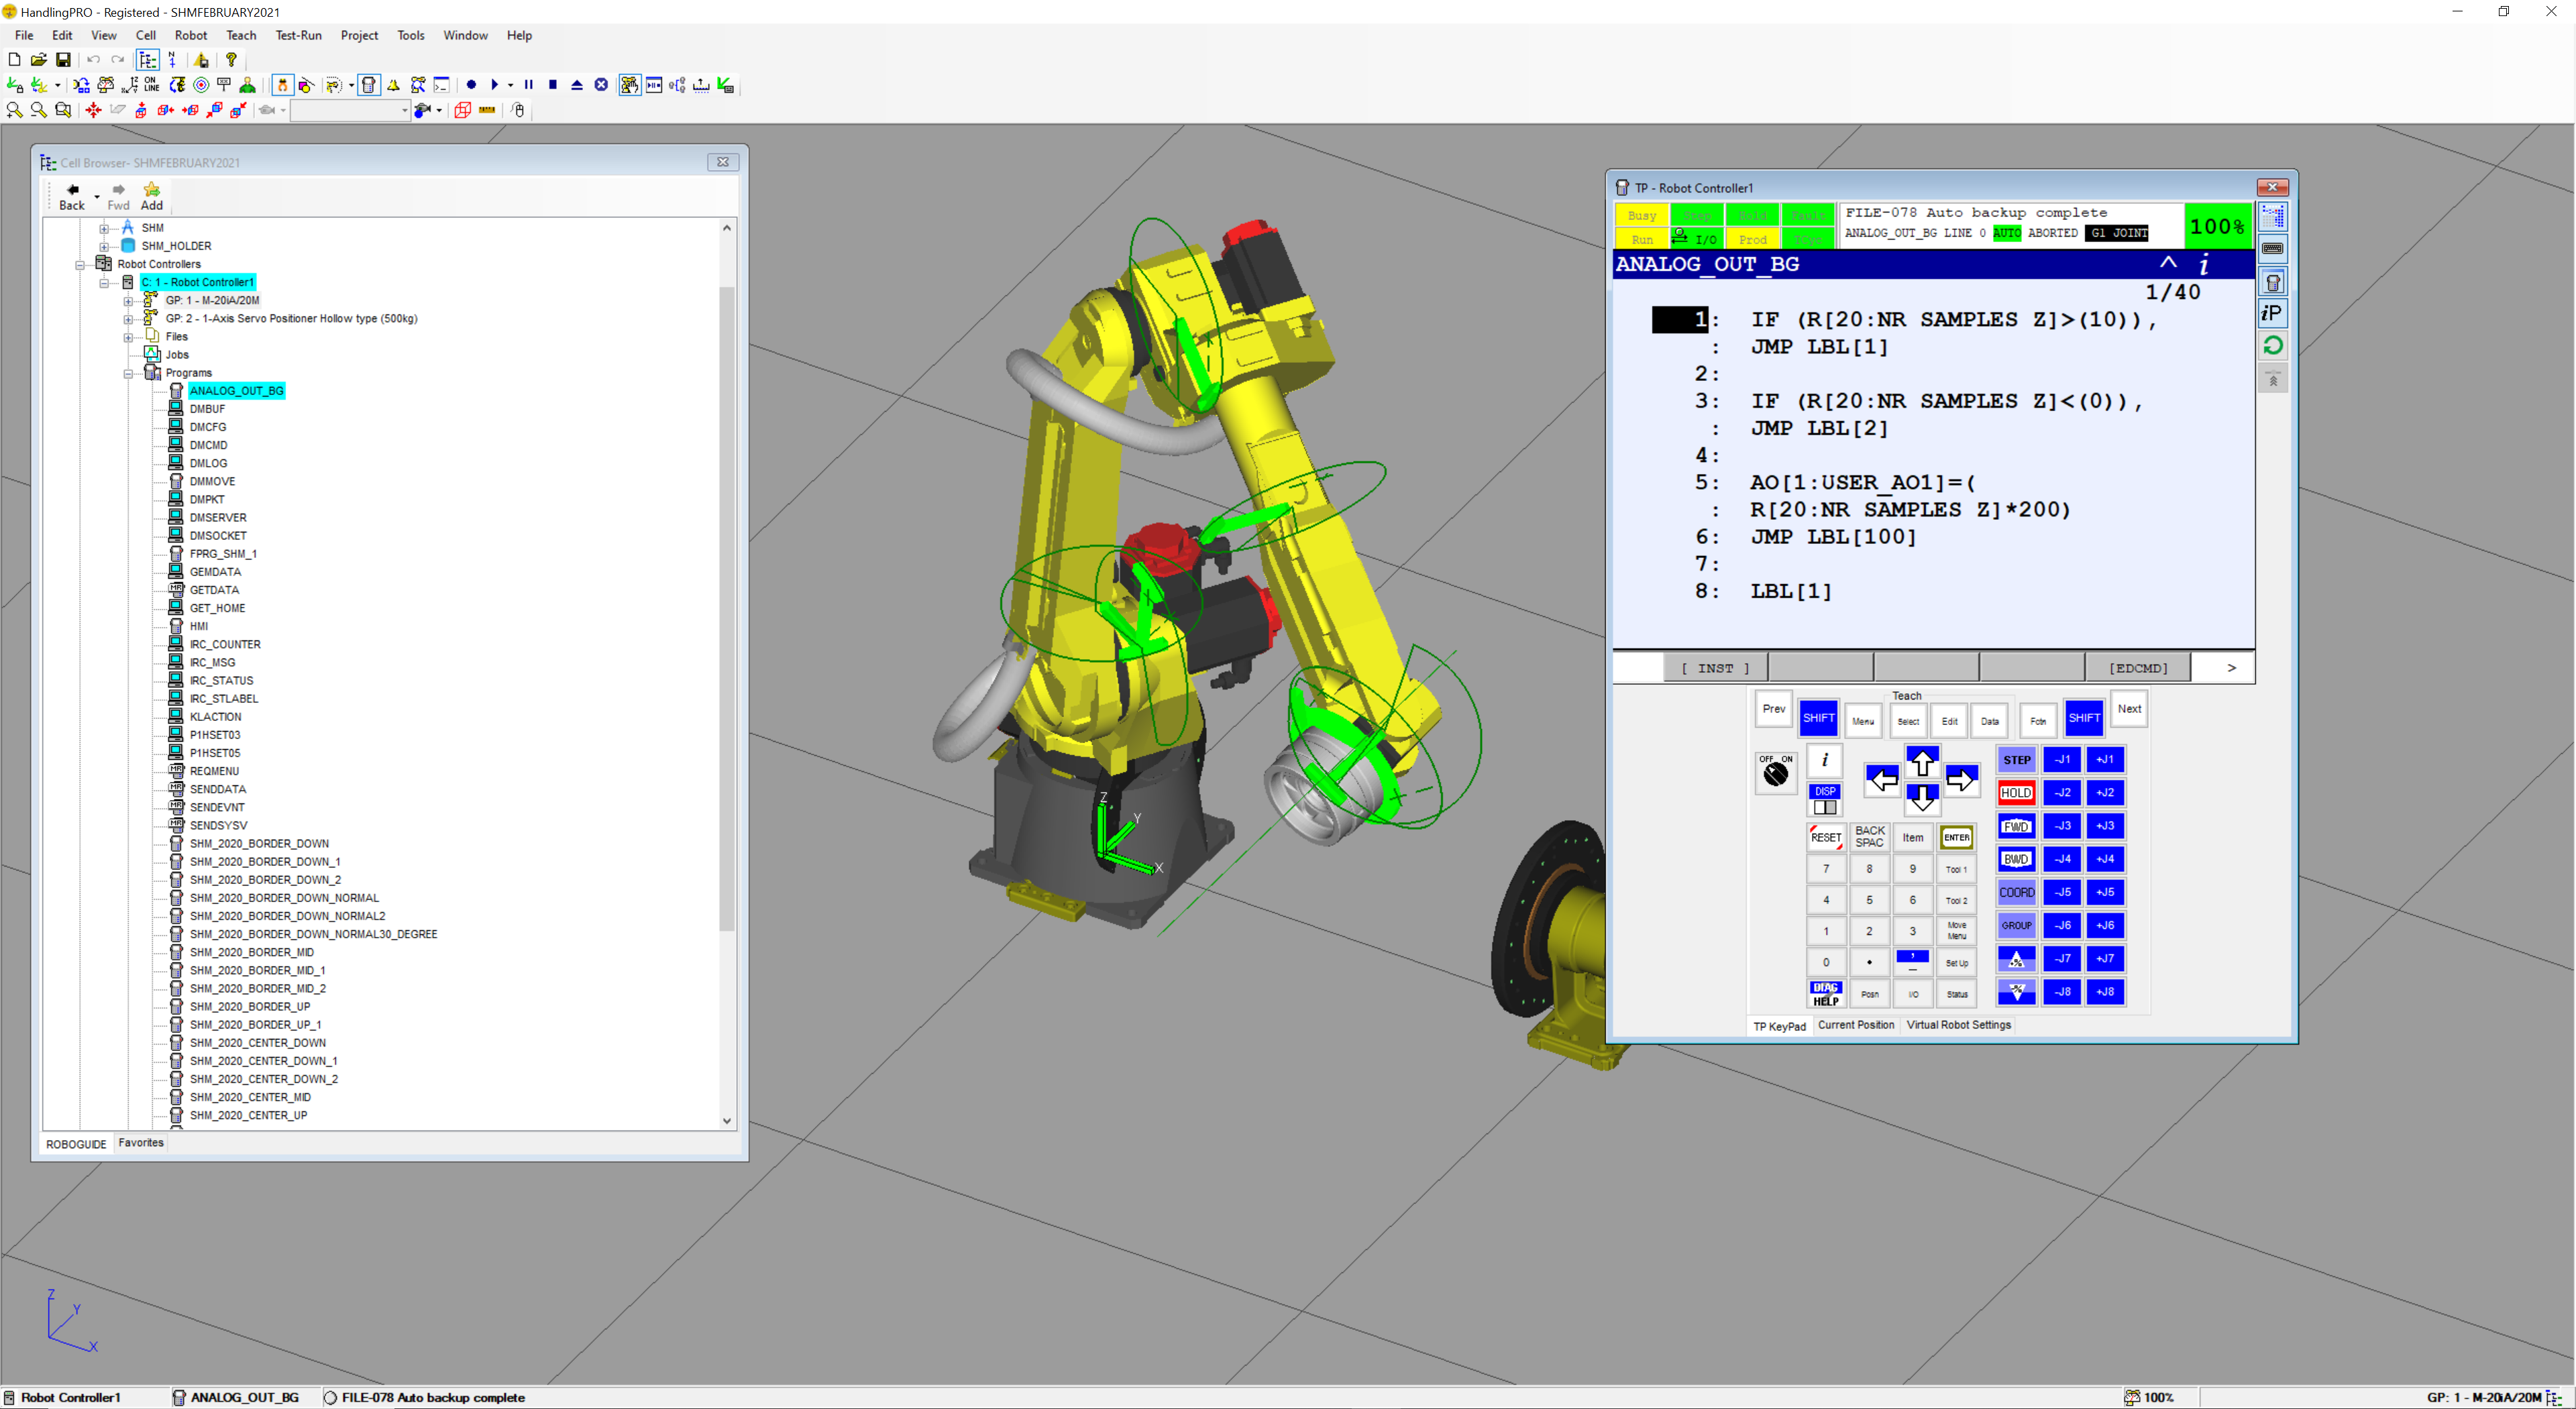
\includegraphics[width=0.9\linewidth]{img/roboguide.PNG}
    \caption{FANUC Roboguide work cell - user interface example.}
    \label{fig:roboguide}
\end{figure}

\subsection{FANUC robots programming languages}

The FANUC company implements two programming languages for programming their robot controllers: Teach Pendant (TP) or KAREL. The Teach Pendant language is mainly used for motion control of the robotic arm and edited via the Pendant. Teach pendant programs are either binary files (\mintinline{shell-session}{.tp} file extension) or can be human-readable ASCII files (\mintinline{shell-session}{.ls} file extension). The KAREL language is a high-level language and does not support robot movements. KAREL is mainly used to implement algorithms. KAREL programs can be only edited using a Personal Computer, and they can not be edited using a Pendant.

\subsection{Compiling a FANUC TP program}

Only a Teach Pendant program in binary format can be run on FANUC controllers. Because RoboDK creates TP programs as human-readable ASCII files, the Teach Pendant programs need to be converted to binary format before uploading them to the robot controller. Two options to convert .ls programs to .tp programs exist:

\begin{enumerate}
\item The ASCII Upload option must be loaded on the robot controller. After upload an (\mintinline{shell-session}{.ls} file to the controller it is automatically converted to a (\mintinline{shell-session}{.tp} file.
\item The program is compiled and uploaded either using the WinOLPC  tools via Roboguide or using the WinOLPC tools directly

\end{enumerate}

\section{Robot machining projects in RoboDK}

The applications of robot machining in the industry are numerous. Some applications include:

\begin{itemize}

    \item milling
    \item drilling
    \item chamfering
    \item deburring

\end{itemize}

RoboDK offers three types of robot manufacturing projects:

\begin{itemize}

    \item Robot machining project
    \item Curve follow project 
    \item Point follow project 

\end{itemize}

This chapter deals with setting up a Curve follow project in RoboDK. In laser shock peening, the laser (the tool) is static, and the robot holds the object. Therefore, a Curve follow project with a constant tool orientation is set up in RoboDK.

\subsection{Setting up a Curve follow project in RoboDK}


\section{RoboDK API for Python}

\section{Installation, Python setup and path settings of RoboDK API}

\section{Modifying a post processor}




\chapter{Testing}

    \input{chapters/5_testing}

\chapter{Discussion}

    \input{chapters/6_discussion}
    
%%%%%%% CONCLUSION CHAPTER %%%%%%%
    
\chapter{Conclusion} % SEM NESAHEJTE!
\addcontentsline{toc}{chapter}{Conclusion} % SEM NESAHEJTE!
%
    Zde napište text úvodu (1-3 strany, nerozdělujte na podkapitoly) nebo jej vložte ze samostatného souboru: např. příkazem \texttt{\textbackslash input\{vnitrek\_zaver.tex\}}.
    
%%%%%%% REFERENCES %%%%%%%

\clearpage  % SEM NESAHEJTE!
\addcontentsline{toc}{chapter}{Reference} % SEM NESAHEJTE!
\printbibliography

\begin{appendices}

    \renewcommand{\chaptermark}[1]{\markboth{#1}{#1}}
    \fancyhead[R]{Appendix \thechapter\ --\ \leftmark}
    \fancyhead[L]{}


    \chapter{Contents of the enclosed CD/DVD}
    \input{appendices/enclosed_cd}

    \chapter{Used software}
    \textbf{\LaTeX} - \href{https://miktex.org/}{https://miktex.org/}\newline
\textbf{RoboDK} - \href{https://robodk.com/}{https://robodk.com/}\newline
\textbf{RoboDK} - \href{https://robodk.com/}{https://robodk.com/}\newline
    
    \chapter{Time schedule of thesis}
    \input{appendices/time_schedule}
    
    \chapter{Project budget}
    The following table lists the thesis's operating budget, including purchases of individual components and orders implemented outside school. Prices include VAT and usually including postage and packaging.

\begin{table}[h!]


        \begin{tabular}{|c | c | c | c |} 
        \hline
            \textbf{Component} & \textbf{No. of components} & \textbf{Price per component} & \textbf{Total price}\\ [0.25ex] 
        \hline\hline
        Repetition Rate (Hz) & 1 & 100 & 100  \\ 
        \hline

        \hline
        \end{tabular}

    
        \caption{Financial budget of the project.}
        \label{litro}

\end{table}

The following table shows the hourly work budget for the production of the model implemented within the school. The table contains abbreviations that mean:

\end{appendices}





%%%%%%%%%%%% PŘÍLOHY PRÁCE %%%%%%%%%%%%
\newpage % SEM NESAHEJTE!
\addcontentsline{toc}{chapter}{Přílohy} % SEM NESAHEJTE!
\appendix % SEM NESAHEJTE!


%%%%%%%%%%%% Příloha A (tj. 1. kapitola v rámci příloh) %%%%%%%%%%%%

\end{document} % SEM NESAHEJTE! Konec.
